\documentclass[a4paper, 11pt]{article}
\usepackage{amsthm}
\usepackage{xspace}
\usepackage{siunitx}
\usepackage{booktabs}
\usepackage{miscdoc,multirow,bigstrut,bigdelim,colortbl}
\usepackage{setspace}
\usepackage{listings}
\usepackage{graphicx}
\usepackage{amsmath}


\begin{document}
\title{HomeWork - 2}
\author{Mustafa Tokat}
\maketitle
\section{Introduction}

\indent First,I would like to thank you very much again for giving me such a great opportunity. 
I am looking forward to the lessons and the many new things I can learn. I must confess that I take pleasure in learning this subject. 
At the same time I am so sorry because my english is not sufficient for writing knowledge rules. 
This is my first time writing something of this length. Indeed I am not used to this situation but I aim to explain myself the best I can. 


Furthermore, I preferred to add to the end of this document to all coding documents. 
I thought you would be distracted while you read if I had done otherwise. 
Therefore you will find the aforementioned documents below.  

\section{Analyze of Problems}
\subsection*{Problem 1}

\textbf{\textit{This polynomial is reducible: p(x) = $x^{5} + x^{4} + 1$ Discover the period(s) of the sequence produced by the LFSR using it as its connection polynomial}}
            

\indent \singlespacing There is a reducible polynomial my hands. This is very important in terms of two. At first, 
this polynomial will not produce maximal period. We know to 2 theorem discovered by Solomon Golf Golomb.
The first of these,if we want to produce an n-bit LFSR, of this polynomial have to have  maximal period. If period of this polynomial is not maximal, 
it can produce each time different sequances and this is the case 2 different DRNG machines can  not run compatible. 

Then we should remember theorems of Solomon Golf Golomb's: 


\newtheorem*{thm}{Golomb's first theorem}
\begin{thm}
    If the connection polynomial (of degree n) of an n-bit LFSR is reducible,then its its period is not maximal  ($\neq$$2^{n}-1$)
\end{thm}

And again let's remember of:

\newtheorem*{thm1}{Golomb's second theorem}
\begin{thm1}
    If the connection polynomial of degree n is a primitive polynomial, then the associated LFSR is maximal, with period $2^{n}-1$.
\end{thm1}
Then we can write: $x^{5}+x^{4}+1$ == ($c_{4}, c_{3}, c_{2}, c_{1}, c_{0} $) == (1,0,0,0,1)
Inital state is important because of this polynomial is not irreducible and primitive polynomial. We will see right now.

% Table generated by Excel2LaTeX from sheet 'Sheet1'
\begin{table}[htbp]
    \centering
    \caption{Initial state for 0, 0, 0, 0, 1, periods of number 23}
      \begin{tabular}{rcccccl}
      \hline
      \multicolumn{1}{c}{($c_{4}, c_{3}, c_{2}, c_{1}, c_{0} $)} & 1     & 0     & 0     & 0     & 1     &  \bigstrut\\
      \hline
      \multicolumn{1}{c}{($s_{4}, s_{3}, s_{2}, s_{1}, s_{0} $)} & 1     & 1     & 1     & 0     & 0     & initial value \bigstrut\\
      \hline
      \multirow{3}[6]{*}{} & 1     & 1     & 1     & 1     & 0     & \multirow{2}[4]{*}{} \bigstrut\\
  \cline{2-6}          & 1     & 1     & 1     & 1     & 1     &  \bigstrut\\
  \cline{2-6}          & 0     & 1     & 1     & 1     & 1     &  \bigstrut\\
  \cline{2-6}          & 1     & 0     & 1     & 1     & 1     &  \bigstrut\\
  \cline{2-6}          & 0     & 1     & 0     & 1     & 1     &  \bigstrut\\
  \cline{2-6}          & 1     & 1     & 0     & 0     & 1     &  \bigstrut\\
  \cline{2-6}          & 0     & 1     & 0     & 0     & 1     &  \bigstrut\\
  \cline{2-6}          & 1     & 0     & 1     & 0     & 1     &  \bigstrut\\
  \cline{2-6}          & 0     & 1     & 0     & 1     & 0     &  \bigstrut\\
  \cline{2-6}          & 0     & 0     & 1     & 0     & 1     &  \bigstrut\\
  \cline{2-6}          & 1     & 0     & 0     & 1     & 0     &  \bigstrut\\
  \cline{2-6}          & 1     & 1     & 0     & 0     & 1     &  \bigstrut\\
  \cline{2-6}          & 0     & 1     & 1     & 0     & 0     &  \bigstrut\\
  \cline{2-6}          & 0     & 0     & 1     & 1     & 0     &  \bigstrut\\
  \cline{2-6}          & 0     & 0     & 0     & 1     & 1     &  \bigstrut\\
  \cline{2-6}          & 1     & 0     & 0     & 0     & 1     &  \bigstrut\\
  \cline{2-6}          & 0     & 1     & 0     & 0     & 0     &  \bigstrut\\
  \cline{2-6}          & 0     & 0     & 1     & 0     & 0     &  \bigstrut\\
  \cline{2-6}          & 0     & 0     & 0     & 1     & 0     &  \bigstrut\\
  \cline{2-6}          & 0     & 0     & 0     & 0     & 1     &  \bigstrut\\
  \cline{2-6}          & 1     & 0     & 0     & 0     & 0     &  \bigstrut\\
  \cline{2-6}          & 1     & 1     & 0     & 0     & 0     &  \bigstrut\\
  \cline{2-7}          & 1     & 1     & 1     & 0     & 0     & Repeat \bigstrut\\
  \cline{2-7}    \end{tabular}%
    \label{tab:addlabel}%
  \end{table}%

  
% Table generated by Excel2LaTeX from sheet 'Sheet1'
\begin{table}[htbp]
    \centering
    \caption{Initial state for 0, 0, 0, 0, 1, periods of number 21}
      \begin{tabular}{ccccccl}
      \hline
      ($c_{4}, c_{3}, c_{2}, c_{1}, c_{0} $) & 1     & 0     & 0     & 0     & 1     &  \bigstrut\\
      \hline
      ($s_{4}, s_{3}, s_{2}, s_{1}, s_{0} $) & 0     & 0     & 0     & 0     & 1     & initial value \bigstrut\\
      \hline
      \multirow{21}[42]{*}{} & 1     & 0     & 0     & 0     & 0     & \multirow{20}[40]{*}{} \bigstrut\\
  \cline{2-6}          & 1     & 1     & 0     & 0     & 0     &  \bigstrut\\
  \cline{2-6}          & 1     & 1     & 1     & 0     & 0     &  \bigstrut\\
  \cline{2-6}          & 1     & 1     & 1     & 1     & 0     &  \bigstrut\\
  \cline{2-6}          & 1     & 1     & 1     & 1     & 1     &  \bigstrut\\
  \cline{2-6}          & 0     & 1     & 1     & 1     & 1     &  \bigstrut\\
  \cline{2-6}          & 1     & 0     & 1     & 1     & 1     &  \bigstrut\\
  \cline{2-6}          & 0     & 1     & 0     & 1     & 1     &  \bigstrut\\
  \cline{2-6}          & 1     & 0     & 1     & 0     & 1     &  \bigstrut\\
  \cline{2-6}          & 0     & 1     & 0     & 1     & 0     &  \bigstrut\\
  \cline{2-6}          & 0     & 0     & 1     & 0     & 1     &  \bigstrut\\
  \cline{2-6}          & 1     & 0     & 0     & 1     & 0     &  \bigstrut\\
  \cline{2-6}          & 1     & 1     & 0     & 0     & 1     &  \bigstrut\\
  \cline{2-6}          & 0     & 1     & 1     & 0     & 0     &  \bigstrut\\
  \cline{2-6}          & 0     & 0     & 1     & 1     & 0     &  \bigstrut\\
  \cline{2-6}          & 0     & 0     & 0     & 1     & 1     &  \bigstrut\\
  \cline{2-6}          & 1     & 0     & 0     & 0     & 1     &  \bigstrut\\
  \cline{2-6}          & 0     & 1     & 0     & 0     & 0     &  \bigstrut\\
  \cline{2-6}          & 0     & 0     & 1     & 0     & 0     &  \bigstrut\\
  \cline{2-6}          & 0     & 0     & 0     & 1     & 0     &  \bigstrut\\
  \cline{2-7}          & 0     & 0     & 0     & 0     & 1     & repeat \bigstrut\\
  \cline{2-7}    \end{tabular}%
    \label{tab:Table 1}%
  \end{table}%

   % Table generated by Excel2LaTeX from sheet 'Sheet1'
\begin{table}[htbp]
    \centering
    \caption{Initial state for 0, 1, 1, 0, 1, periods of number 3}
      \begin{tabular}{ccccccl}
      \hline
      ($c_{4}, c_{3}, c_{2}, c_{1}, c_{0} $) & 1     & 0     & 0     & 0     & 1     &  \bigstrut\\
      \hline
      ($s_{4}, s_{3}, s_{2}, s_{1}, s_{0} $) & 0     & 1     & 1     & 0     & 1     & initial value \bigstrut\\
      \hline
      \multirow{3}[6]{*}{} & 1     & 0     & 1     & 1     & 0     & \multirow{2}[4]{*}{} \bigstrut\\
  \cline{2-6}          & 1     & 1     & 0     & 1     & 1     &  \bigstrut\\
  \cline{2-7}          & 0     & 1     & 1     & 0     & 1     & repeat \bigstrut\\
  \cline{2-7}    \end{tabular}%
    \label{tab:Table 2}%
  \end{table}%
    % Table generated by Excel2LaTeX from sheet 'Sheet1'
\begin{table}[htbp]
    \centering
    \caption{Initial state for 1, 1, 1, 0, 1, periods of number 7}
      \begin{tabular}{rcccccl}
      \hline
      \multicolumn{1}{c}{($c_{4}, c_{3}, c_{2}, c_{1}, c_{0} $)} & 1     & 0     & 0     & 0     & 1     &  \bigstrut\\
      \hline
      \multicolumn{1}{c}{($s_{4}, s_{3}, s_{2}, s_{1}, s_{0} $)} & 1     & 1     & 1     & 0     & 1     & initial value \bigstrut\\
      \hline
      \multirow{3}[6]{*}{} & 0     & 1     & 1     & 1     & 0     & \multirow{2}[4]{*}{} \bigstrut\\
  \cline{2-6}          & 0     & 0     & 1     & 1     & 1     &  \bigstrut\\
  \cline{2-6}          & 1     & 0     & 0     & 1     & 1     &  \bigstrut\\
  \cline{2-6}          & 0     & 1     & 0     & 0     & 1     &  \bigstrut\\
  \cline{2-6}          & 1     & 0     & 1     & 0     & 0     &  \bigstrut\\
  \cline{2-6}          & 1     & 1     & 0     & 1     & 0     &  \bigstrut\\
  \cline{2-7}          & 1     & 1     & 1     & 0     & 1     & repeat \bigstrut\\
  \cline{2-7}    \end{tabular}%
    \label{tab:Table 3}%
  \end{table}%

  

\textbf{Result: I tried 4 different inital state values. As it seen from tables, 4 different initial state values produced 4 different periods. Also, if given polynomial were primitive polynomial whatsoever 
initial state value would produce the same periods, in unique period number $2^{5}-1$ = 31.}

\subsection*{Problem 2}
\textbf{\textit{Prove that p(x) = $x^{10} + x^{3}$ + 1 is primitive over GF(2).}} 

\singlespacing A polynomial have to be irreducible for primitive polynomial. We can understand that; at first, given polynomial is divided with $x^{e}+1$. After, n value continues 
  to increment 1 by e each time, until divided without remainder. However, (e) value can be divided with a few number as without remainder. But we want \underline{the first value}
   to satisfy e = $2^{n}-1$. We can do it that:
   
starting from n;

\setstretch{2.5}\begin{center} 1. trying: $\frac{2^e-1}{x^{10} + x^{3}+1}$

 2. trying: $\frac{2^{e+1}-1}{x^{10} + x^{3}+1}$

 3. trying: $\frac{2^{e+2}-1}{x^{10} + x^{3}+1}$

This process continues until e = $2^{n}-1$ first value of e.
\end{center}

\setstretch{6}

After briefly explaining the process, I want to present my Python codes.
\singlespacing


%\noindent import numpy as np\\
%from sympy import prem\\
%from sympy.abc import x\\

%\noindent power1 = int(input('Power1: '))\\
%power2 = int(input('Power2: '))\\
%range1 = int(input('Range1: '))\\
%range2 = int(input('Range2: '))\\

%\noindent def primitiveTest():\\
%\indent    for i in range(range1,range2):\\
%\indent \indent \tiny m =  ((prem (x**i + 1, x**power1 + x**power2 + 1, modulus = 2) == 0) and i == 2**power1 - 1)
%\indent \indent \normalsize if m == True:\\
%indent \indent \indent print(i)\\
%\indent \indent      else:\\
%\indent \indent \indent            i + 1\\
%\indent\indent\indent           print('Not Primitive')\\
       

%\noindent primitiveTest()\\%%

\lstset{language=Python}
\lstset{frame=lines}
\lstset{caption={My code particle which test to whether primitive polynomial}}
\lstset{label={lst:code_direct}}
\lstset{basicstyle=\footnotesize}
\begin{lstlisting}
import numpy as np
from sympy import prem
from sympy.abc import x
    
power1 = int(input('Power1: '))
power2 = int(input('Power2: '))
range1 = int(input('Range1: '))
range2 = int(input('Range2: '))
    
def primitiveTest():
       
    for i in range(range1,range2):
            
        m = ((prem (x**i + 1, x**power1 + x**power2 + 1, modulus = 2) == 0) and 
        i == 2**power1 - 1)
    
        if m == True :
     
            print(i)
    
        else:
            i + 1
            print('Not Primitive')
           
    
primitiveTest()
\end{lstlisting}

\begin{figure}[!h]
    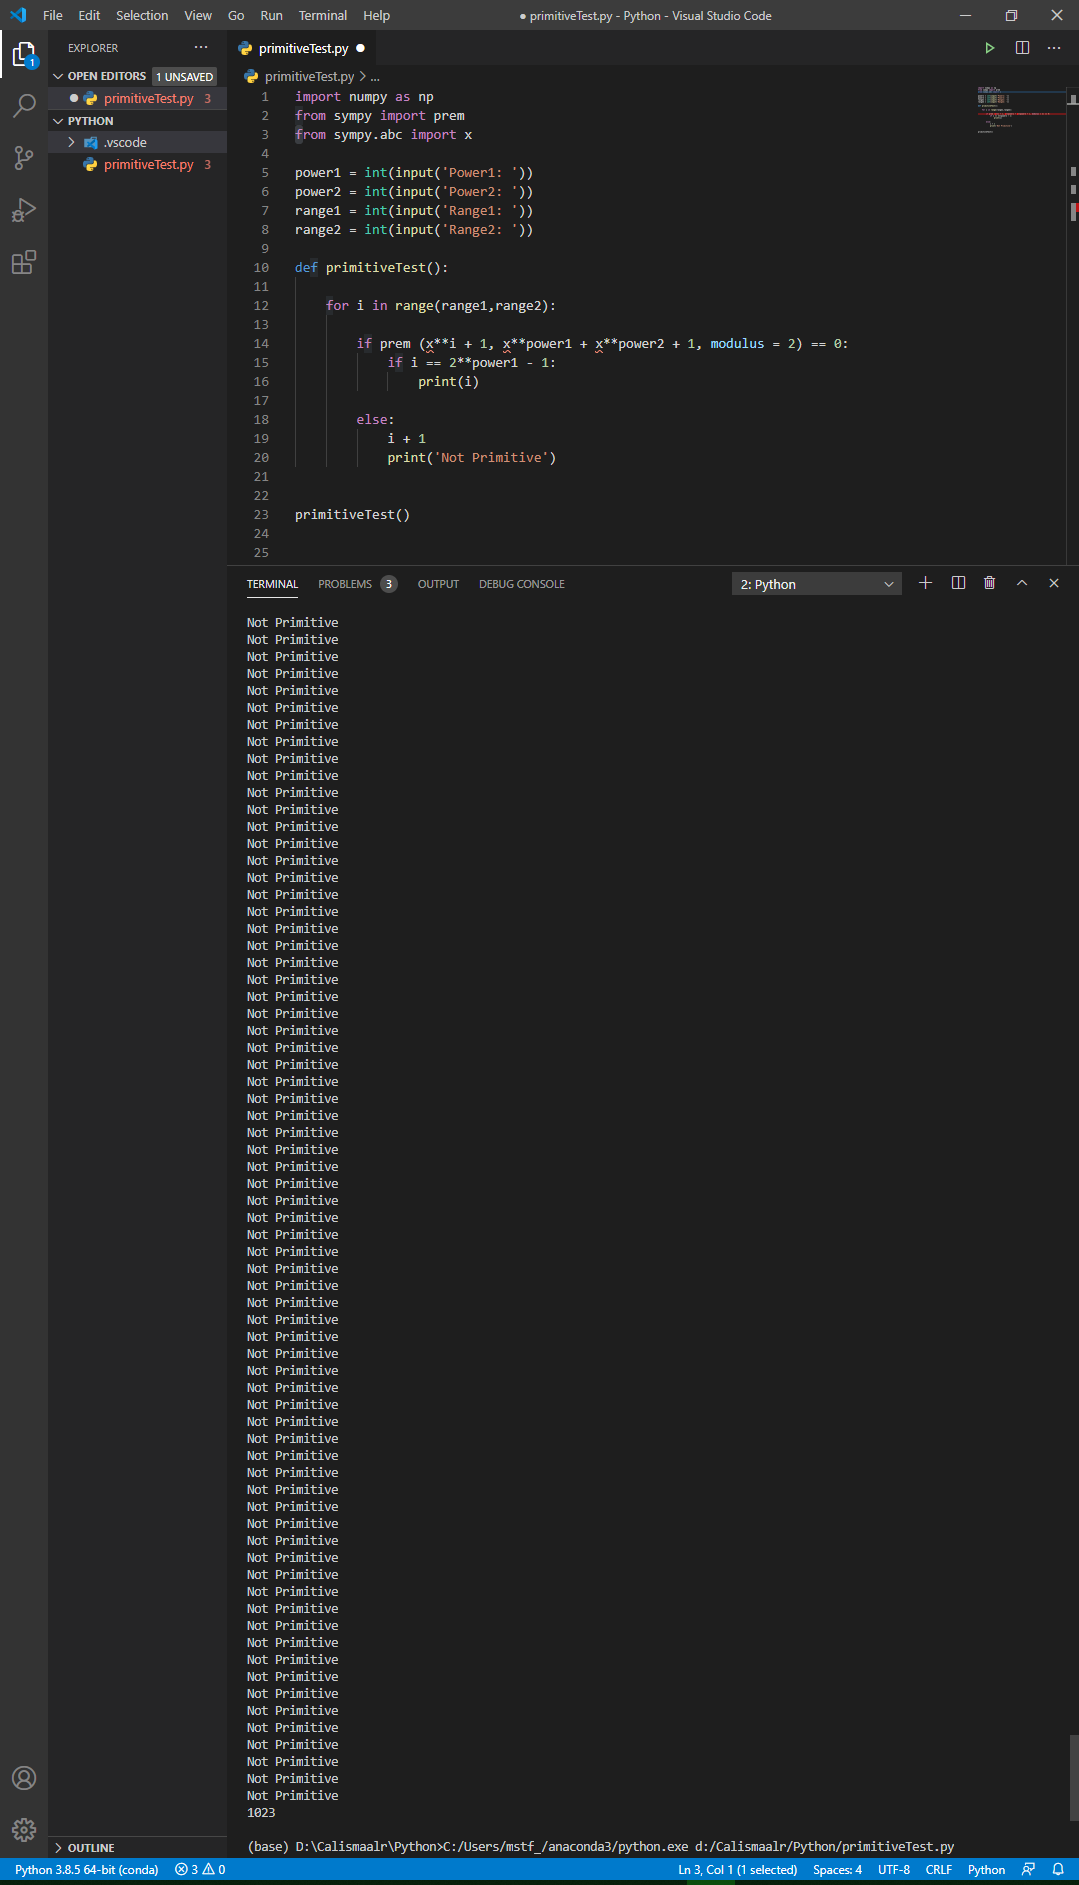
\includegraphics[width=\linewidth]{PrimitiveTest.png}
    \caption{$x^{10} + x^{3}$ + 1 is a primitive polynomial}
    \label{fig:boat1}
\end{figure}
\setstretch{1,5}
\textbf{Result: $x^{10} + x^3 + 1$ is a primitive polynomial according to test result.(Figure 1)} 

\newpage\subsubsection*{Problem 3}
\textbf{\textit{Consider the following sequence, and construct the smallest LSFR producing this sequence
using the Berlekamp-Massey algorithm: 1001101001000010101110110001111100110}}

\singlespacing Indeed we will use to advantage that LFSR has a linear equation system, of course, according to adversary.
So, we need to have two things. 
\begin{itemize}
    \item to r values
    \item the sequence that I had obtained before(as $s_{0}, s_{1}, s_{n}$)
\end{itemize}
We will  use a kind of deductive method. We actually will think as matrix system.  %neden 1 den baslamadigini ekle

 \begin{center} 
    \setstretch{2}
     $s_{n} = c_{n-1}s_{n-1} + c_{n-2}s_{n-2} +.......+ c_{1}s_{1} + c_{0}s_{0}$
     $s_{n+1} = c_{n-1}s_{n} + c_{n-2}s_{n-1} +.......+ c_{1}s_{2} + c_{0}s_{1}$
     $s_{n+2} = c_{n-1}s_{n+1} + c_{n-2}s_{n} +.......+ c_{1}s_{3} + c_{0}s_{2}$\\
     .\\
      .\\
      .\\
      $s_{2n-2} = c_{n-1}s_{2n-3} + c_{2n-4}s_{n} +.......+ c_{1}s_{n-1} + c_{0}s_{n-2}$\\
      $s_{2n-1} = c_{n-1}s_{2n-2} + c_{2n-3}s_{n} +.......+ c_{1}s_{n} + c_{0}s_{n-1}$\\

      
 \end{center} 
 

 If we think of it as a matrix we will need 's' values of 2 times the 'c' values. 
 We know that 'r' values actually mean of 'c' values. And we 
 will seek  'n' values with exhaustive method. I sought n = 2, n = 3, n = 4, and I could not validate with other 's' values. I did not try n = 1 because  it would produce all 0 or all 1.
I found n = 5 bit LFSR construct according to the code I prepared, which I will add end of my homework. Therefore I will give to following example according to n = 5.

I need to do that:

\begin{center}
  \begin{equation*}
     \begin{bmatrix}
      s_{4} & s_{3} & s_{2} & s_{1} & s_{0}\\
      s_{5} & s_{4} & s_{3} & s_{2} & s_{1}\\
      s_{6} & s_{5} & s_{4} & s_{3} & s_{2}\\
      s_{7} & s_{6} & s_{5} & s_{4} & s_{3}\\
      s_{8} & s_{7} & s_{6} & s_{5} & s_{4}\\
    \end{bmatrix} 
    *
    \begin{bmatrix}
      c_{4}\\  c_{3}\\  c_{2}\\ c_{1}\\  c_{0}
    \end{bmatrix}
    =
    \begin{bmatrix}
      s_{5}\\  s_{6}\\  s_{7}\\ s_{8}\\  s_{9}
    \end{bmatrix}
  \end{equation*}
\end{center}


 So, I will identify to Python and find to ($c_{4}, c_{3}, c_{2}, c_{1}, c_{0} $):

\begin{center}
  \begin{equation*}
    \begin{bmatrix}
      c_{4}\\  c_{3}\\  c_{2}\\ c_{1}\\  c_{0}
    \end{bmatrix}
    =
    \begin{bmatrix}
     0\\  1\\  0\\ 0\\  1
    \end{bmatrix}
  \end{equation*}
\end{center}

I need to validation, 'c' values always same, and that:

\begin{center}
  \begin{equation*}
     \begin{bmatrix}
      s_{19} & s_{18} & s_{17} & s_{16} & s_{15}\\
      s_{20} & s_{19} & s_{18} & s_{17} & s_{16}\\
      s_{21} & s_{20} & s_{19} & s_{18} & s_{17}\\
      s_{22} & s_{21} & s_{20} & s_{19} & s_{18}\\
      s_{23} & s_{22} & s_{21} & s_{20} & s_{19}\\
    \end{bmatrix} 
    *
    \begin{bmatrix}
      c_{4}\\  c_{3}\\  c_{2}\\ c_{1}\\  c_{0}
    \end{bmatrix}
    =
    \begin{bmatrix}
      s_{20}\\  s_{21}\\  s_{22}\\ s_{23}\\  s_{24}
    \end{bmatrix}
  \end{equation*}
\end{center}

I check it and I see that ($s_{20} , s_{21}, s_{22}, s_{23}, s_{24}$) = (1, 0, 1, 1, 0)\singlespacing


\noindent\textbf{Result: n = 5 the smallest LSFR producing according to this sequence.(Figure 2)}\singlespacing

\singlespacing\noindent P.S.: In order for you not to be disturbed while reading, I will only share the relevant code snippets, you can find all of them in the attachment.


\begin{figure}[!h]
  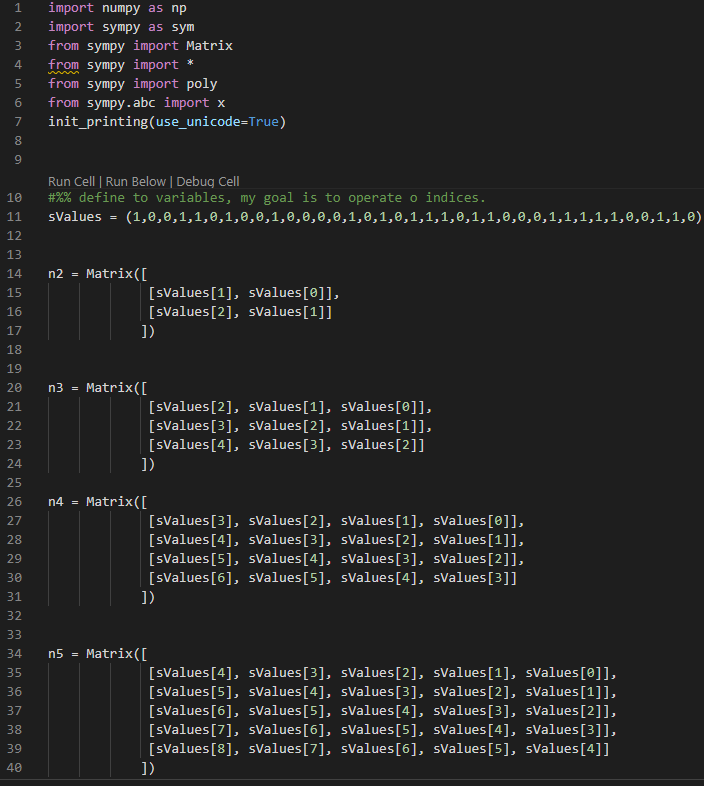
\includegraphics[width=\linewidth]{findToConnPoly__Define_Variable.png}
  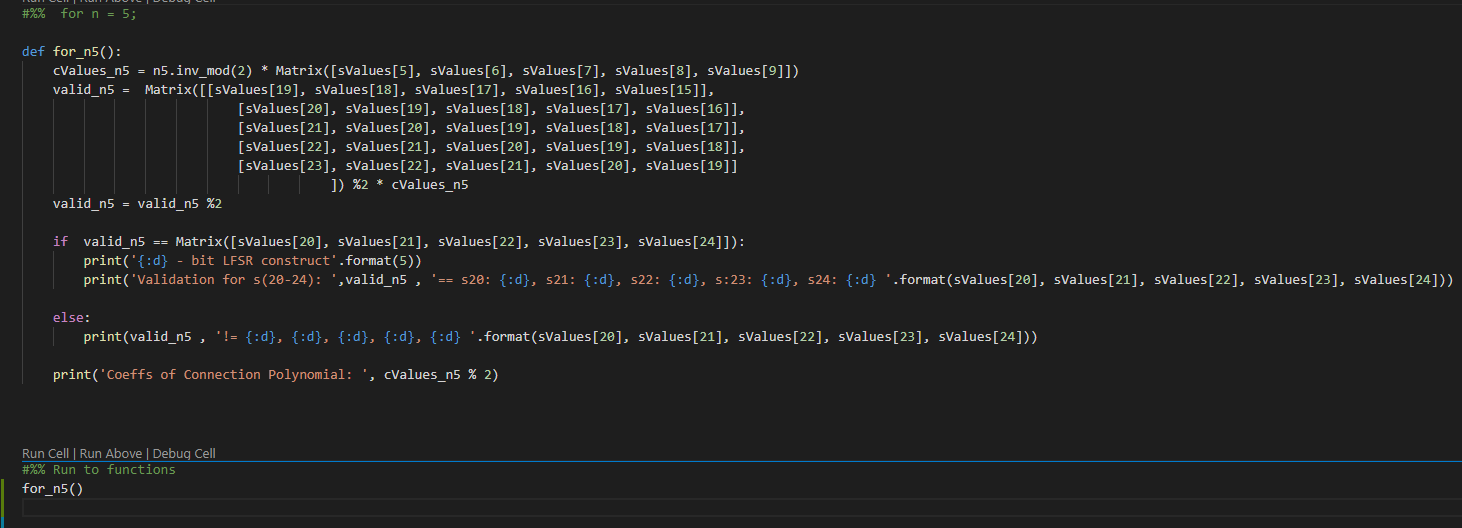
\includegraphics[width=\linewidth]{findToConnPoly_Function.png}
  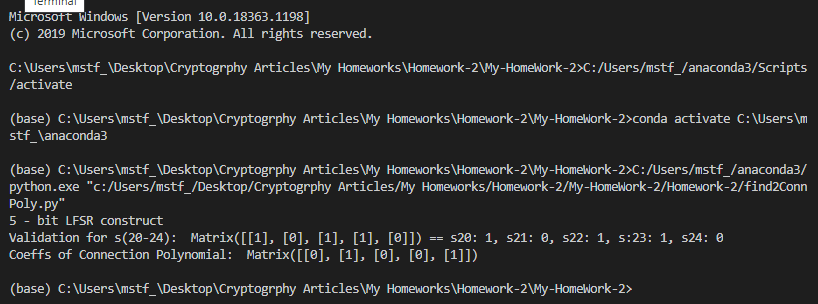
\includegraphics[width=\linewidth]{findToConnPoly_Result.png}
  \caption{My codes for 5 bit LFSR construct according to given sequence }
  \label{fig:resim}
\end{figure}


\end{document}
